\chapter{Обсуждение экспериментальных результатов} \label{chapt4}
В данной главе представлены результаты экспериментальных исследований структуры и квантовомеханических расчётов синтетического теннантита Cu\textsubscript{12}As\textsubscript{4}S\textsubscript{13}, исследование зависимостей намагниченности в диапазоне температур от 2 до 350~К и спектров комбинационного рассеяния света для соединений при комнатной температуре Cu\textsubscript{12}As\textsubscript{4}S\textsubscript{13}, Cu\textsubscript{12}Sb\textsubscript{4}S\textsubscript{13}, Cu\textsubscript{3}AsSe\textsubscript{3} и Cu\textsubscript{3}SbSe\textsubscript{3}. А также измерение телоёмкости в диапазоне температур от 4 до 350~К и результаты моделирования теплоёмкости для Cu\textsubscript{12}As\textsubscript{4}S\textsubscript{13} и Cu\textsubscript{3}AsSe\textsubscript{3}.
Экспериментальные результаты рассматриваются в контексте опубликованных научных литературных данных. Кроме того, в главе отмечаются пути дальнейшего исследования синтезированных соединений.

Анализ результатов начинается с обсуждения особенностей структуры синтетического теннантита в диапазоне температур от 100 до 300~К, особенностей экспериментальной и расчётной теплоёмкости в диапазоне температур от 2 до 350~К и закономерностей изменения магнитных свойств при изовалентном замещении в сложных халькогенидах меди в диапазоне температур от 2 до 350~К.

\section{Рентгеноструктурный анализ синтетического теннантита и результаты квантовомеханических расчётов} \label{sect4_1}

По результатам рентгеноструктурного анализа монокристаллического образца синтетического теннантита Cu\textsubscript{12}As\textsubscript{4}S\textsubscript{13} при комнатной температуре обнаружено, что значение суммы заселённостей позиций атомов Cu2 и Cu21 составляет 1, а не 1.04 как опубликовано ранее\cite{Makovicky_2006}.
Полученные результаты показывают, что на структурную формулу синтетического теннантита приходится 12 атомов меди, а не 12.5.
Таким образом, лавесовский полиэдр состоит из 6 атомов меди.
Разное значение эллиптичности рядов, определенное при анализе плоскости (011) атомарного изображения монокристаллического образца синтетического теннантита Cu\textsubscript{12}As\textsubscript{4}S\textsubscript{13} (Рис.~\ref{img:mic}), говорит в пользу существования позиции меди Cu21 в структуре теннантите, что согласуется с результатами рентгеноструктурного анализа описанного выше. Произвести количественный анализ изображения не удалось.



На рисунке~\ref{img:xray} представлены: величина заселённости позиций атома Cu2 и изменение значения коэффициента атомарного смещения для позиции атома S2 в диапазоне температур от 85 до 293~К. Аномальное изменение значения коэффициента атомарного смещения для позиции атома S2, показывает наличие фазового перехода второго рода в диапазоне от 115 до 180 К.

\begin{figure}[ht]
  \begin{minipage}[ht]{0.5\linewidth}\centering
    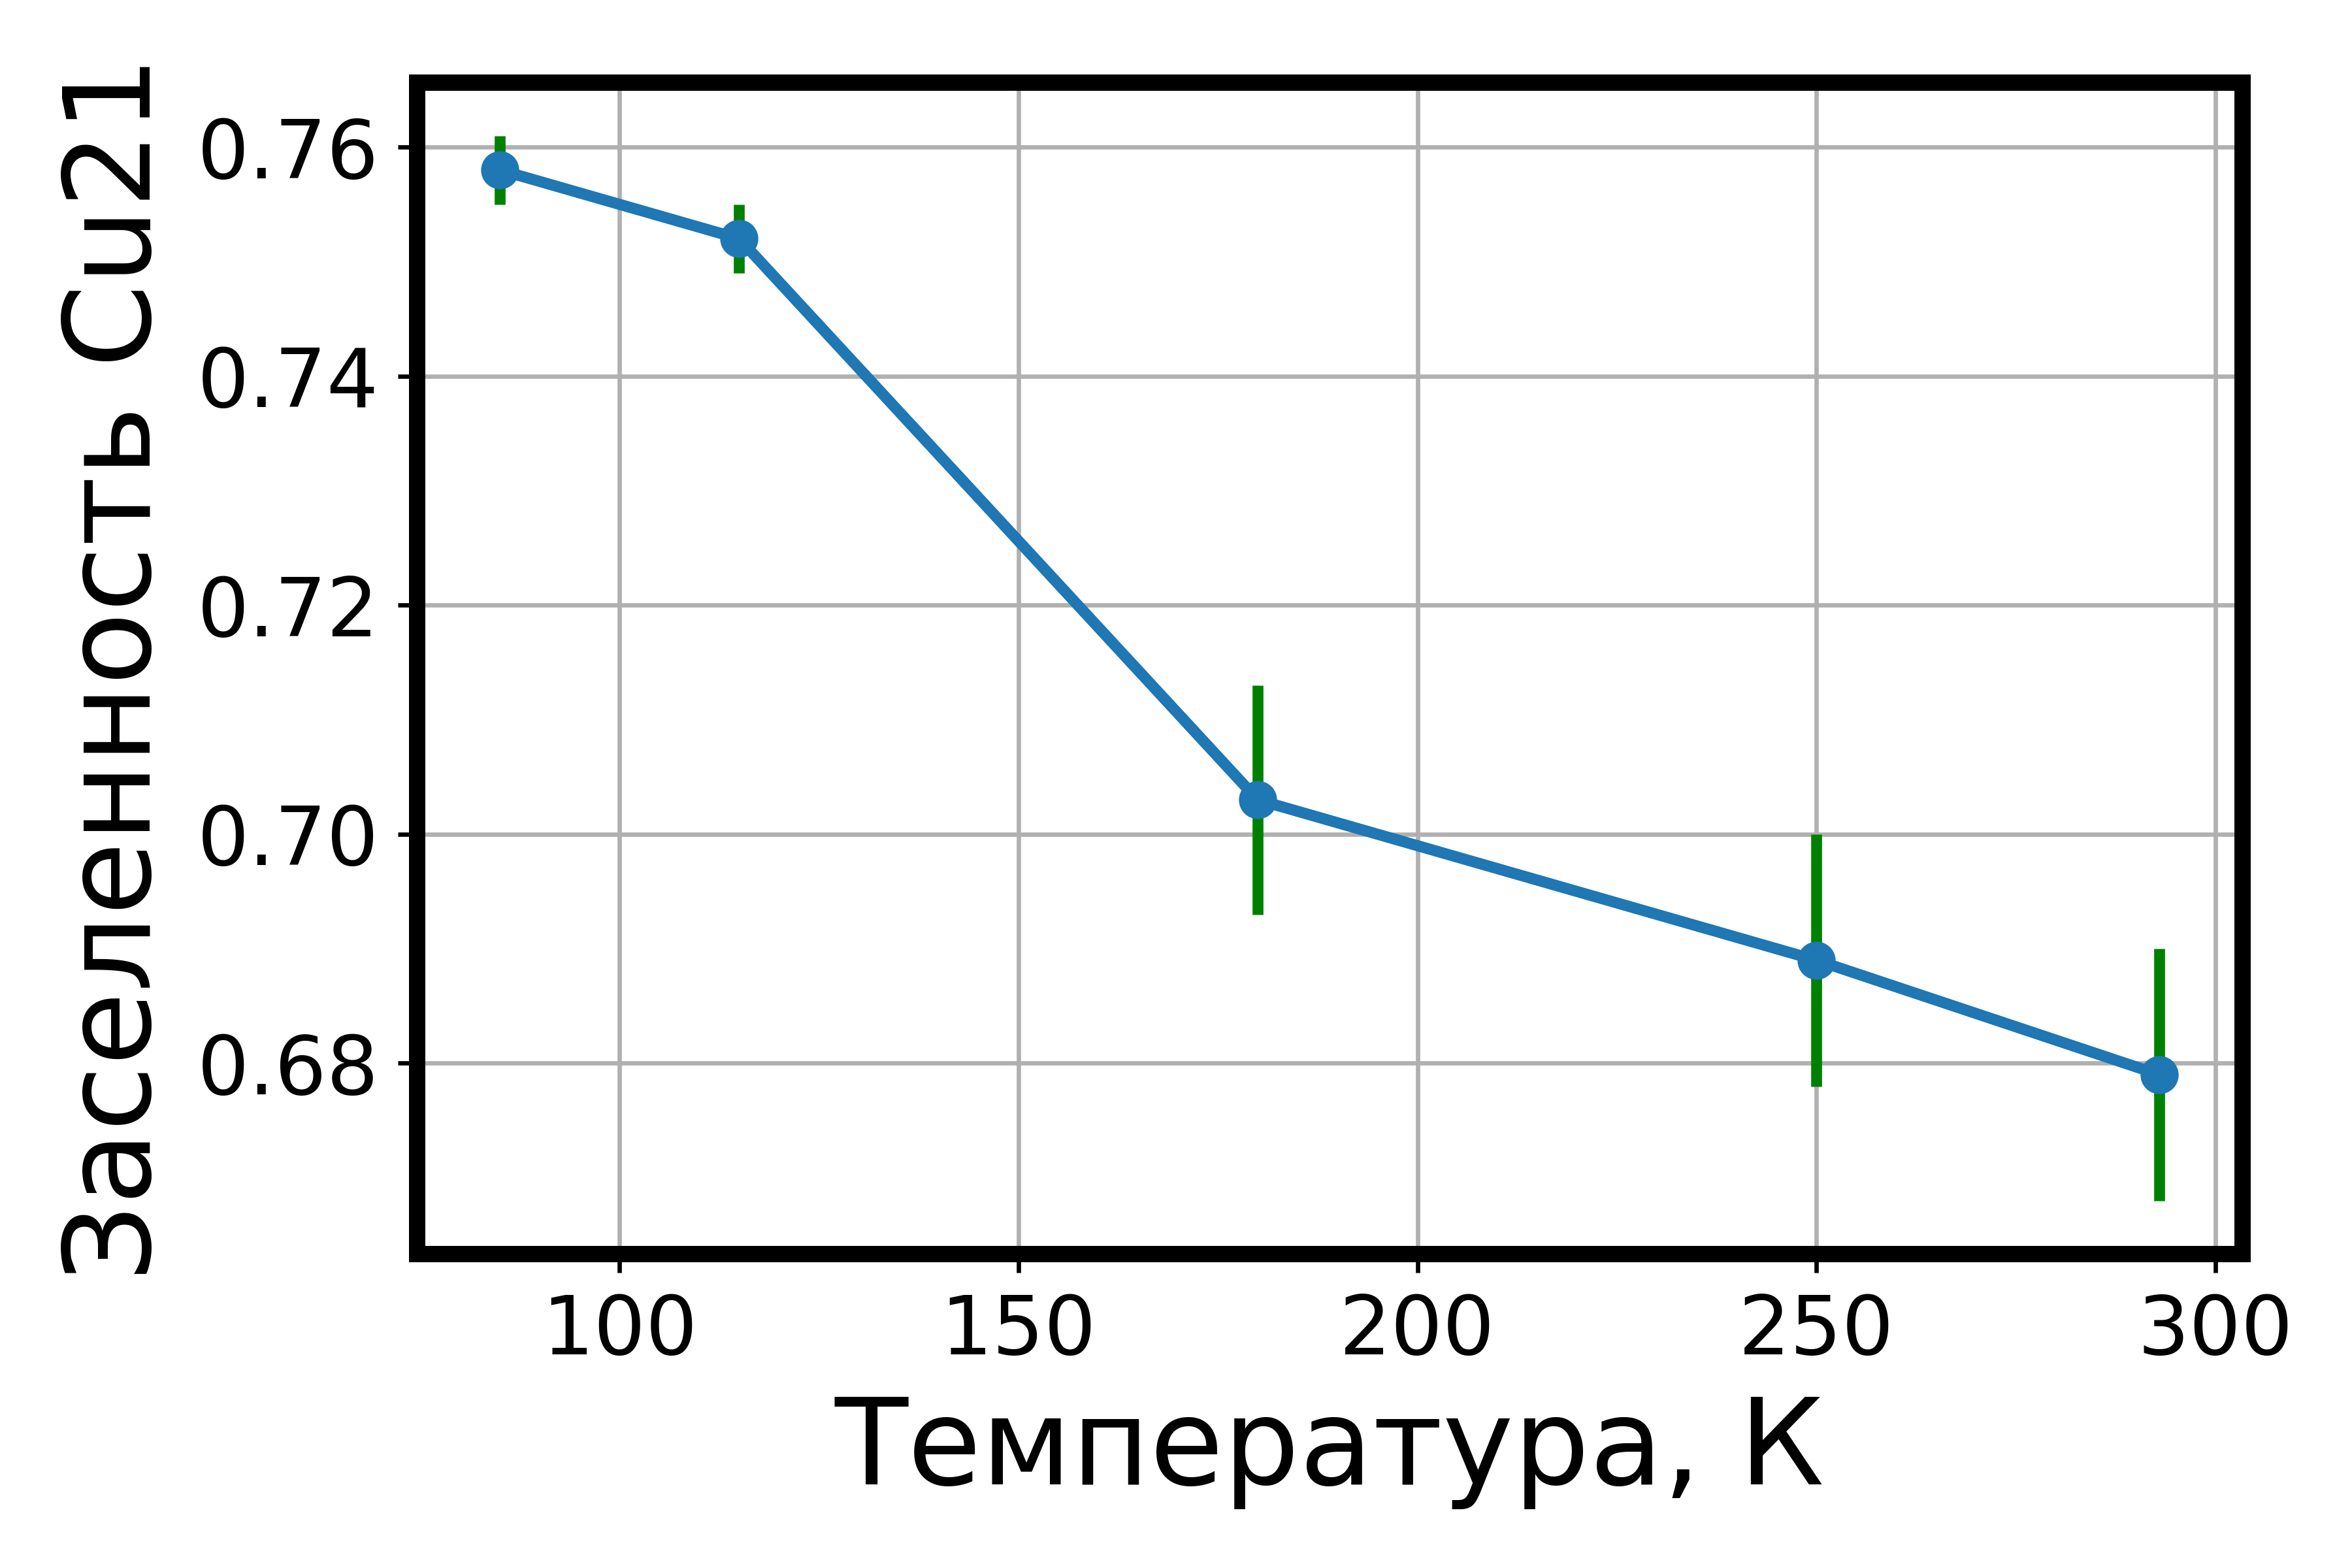
\includegraphics[width=0.9\linewidth]{structure_occCu2} \\ а)
  \end{minipage}
  \hfill
  \begin{minipage}[ht]{0.5\linewidth}\centering
    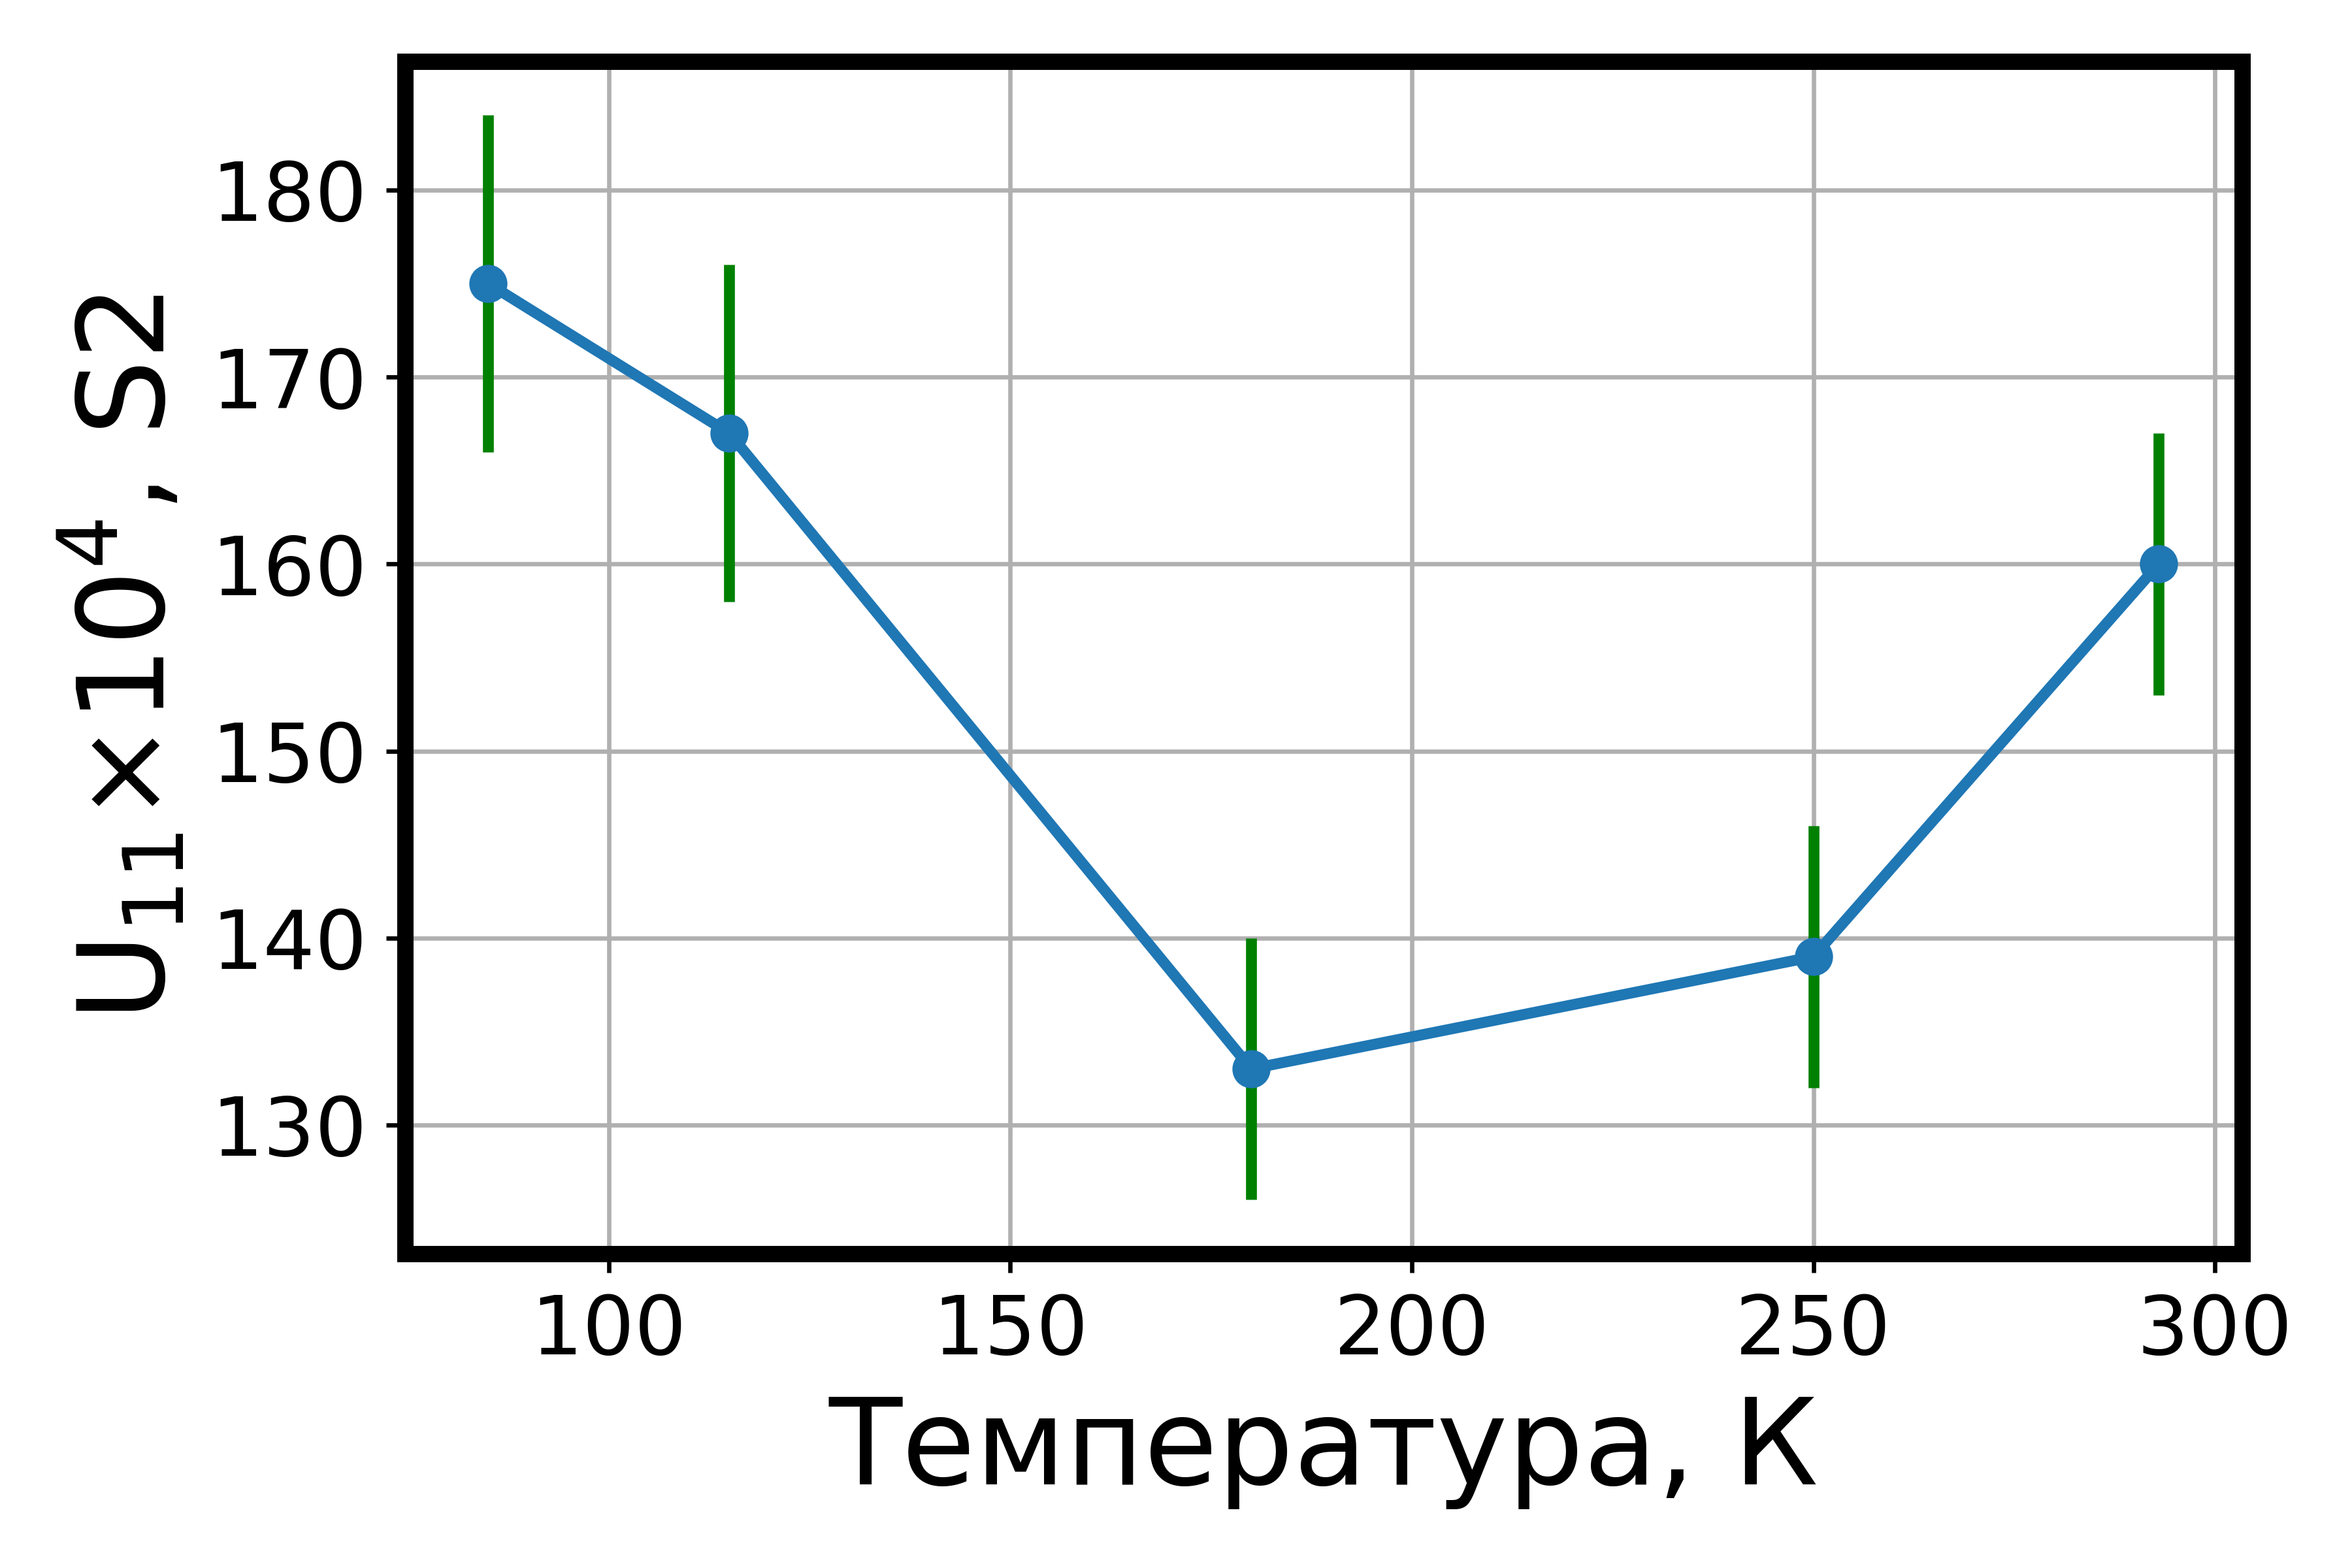
\includegraphics[width=0.9\linewidth]{structure_Ueq} \\ б)
  \end{minipage}

      \caption[Значение заселённости позиции атома Cu2 (а) и изменение значения коэффициента атомарного смещения для позиции атома S2 (б) в диапазоне температур от 85 до 293~К синтетического теннантита Cu\textsubscript{12}As\textsubscript{4}S\textsubscript{13}]{Значение заселённости позиции атома Cu2 (а) и изменение значения коэффициента атомарного смещения для позиции атома S2 (б) в диапазоне температур от 85 до 293~К синтетического теннантита Cu\textsubscript{12}As\textsubscript{4}S\textsubscript{13}}
    \label{img:xray}
\end{figure}

Рисунок \ref{img:xray2} представляет собой изображения распределений электронной плотности синтетического теннантита Cu\textsubscript{12}As\textsubscript{4}S\textsubscript{13} при температуре 293~(а) и 85~(б)~К в плоскости (011). По форме линий электронной плотности видно, что происходит полное разделение позиций Cu2 и Cu21. При комнатной температуре расстояние между Cu2 и Cu21 составляет 1.027(6)~$\angstrom$, при 85~К --- 1.108(5)~$\angstrom$. Расчёт энергий ФМ, АФМ, ПМ и диамагнитного состояний для экспериментально полученных структур показывает, что АФМ упорядочение в экспериментальной структуре при 85~К энергетически более выгодно, чем ферро- или пара- или диамагнитное состояния при этой же температуре. Для экспериментальной структуры при 293~К ФМ, АФМ, ПМ конфигурации имеют одинаковую (до 4 знака) энергию, что указывает на их одинаковую выгодность.

\begin{figure}[ht]
  \begin{minipage}[ht]{0.5\linewidth}\centering
    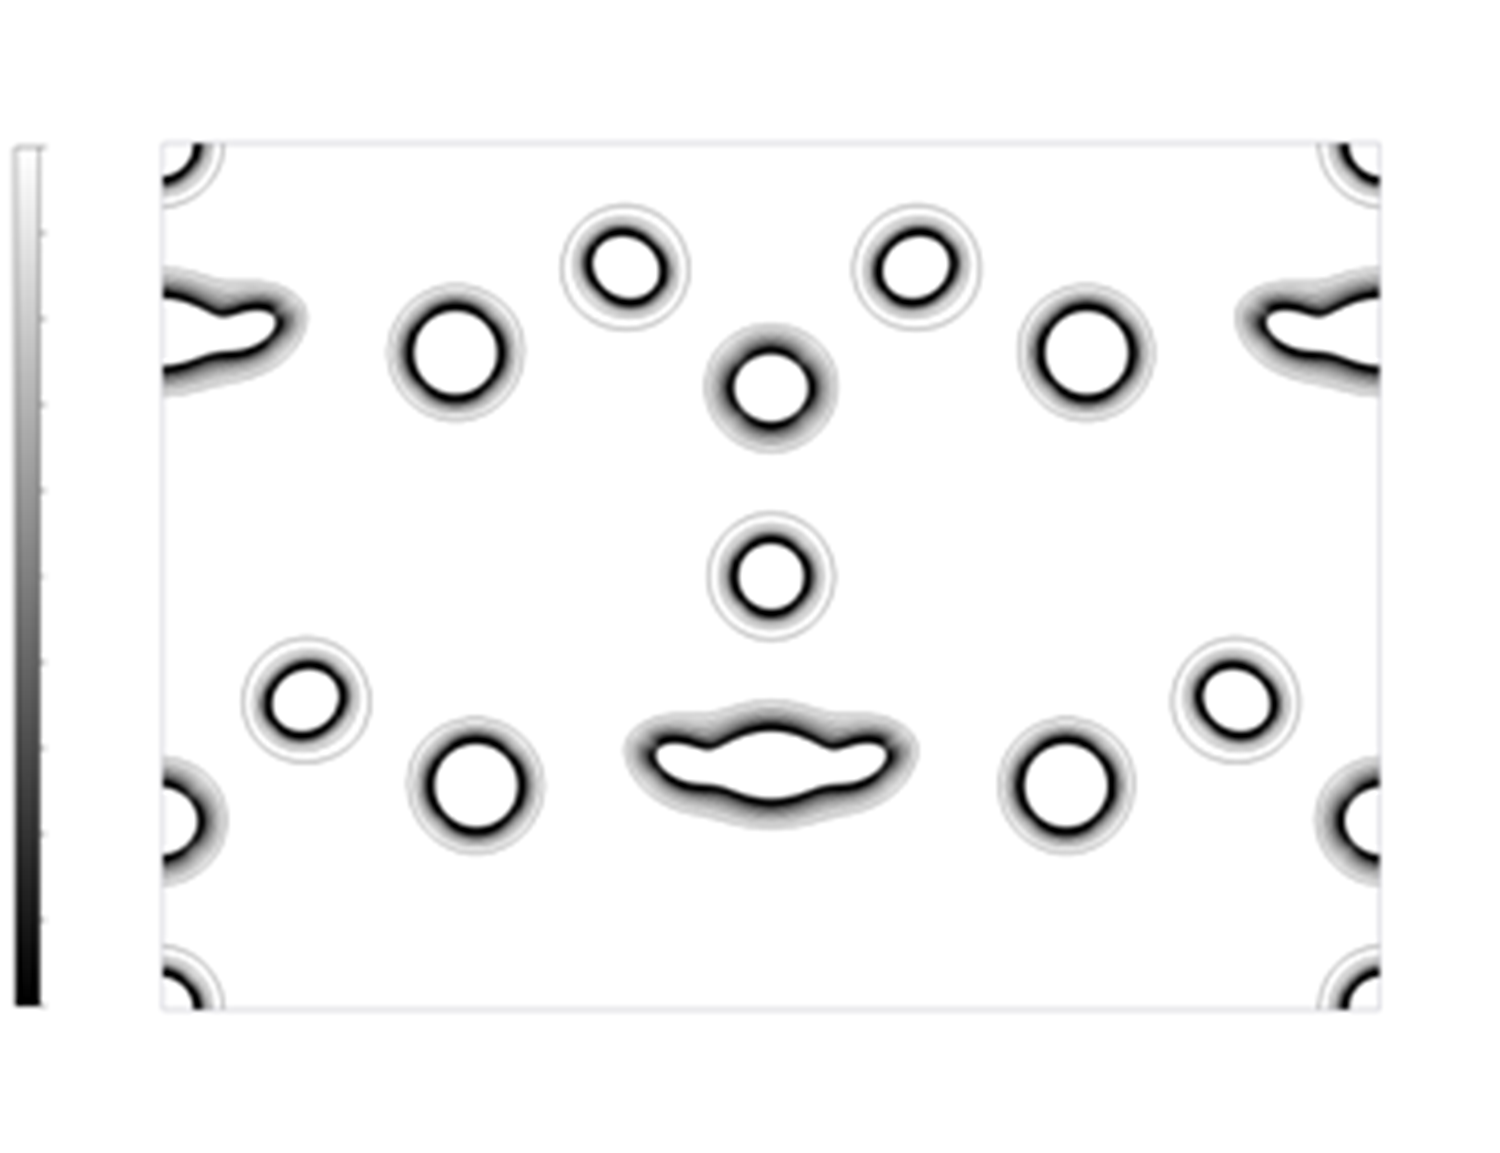
\includegraphics[width=0.9\linewidth]{Electron_density_293.png} \\ а)
  \end{minipage}
  \hfill
  \begin{minipage}[ht]{0.5\linewidth}\centering
    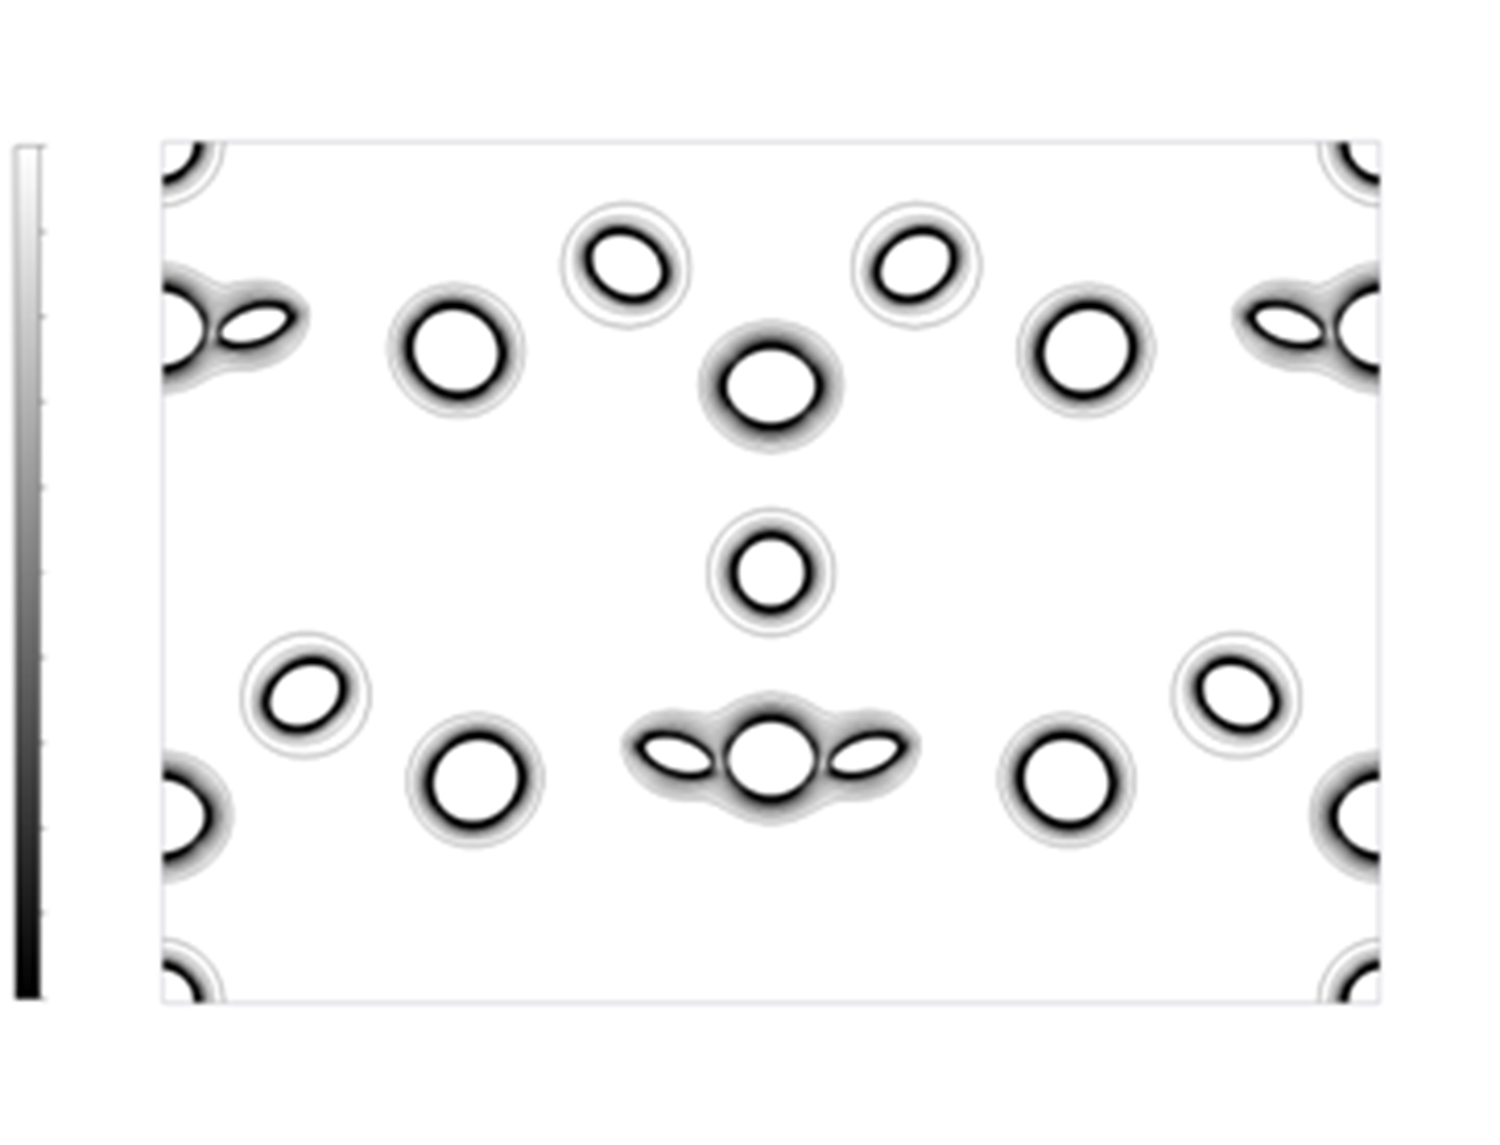
\includegraphics[width=0.9\linewidth]{Electron_density_85.png} \\ б)
  \end{minipage}

      \caption[Распределение электронной плотности при температуре 293~(а) и 85~(б)~К в плоскости (011) синтетического теннантита Cu\textsubscript{12}As\textsubscript{4}S\textsubscript{13}]{Распределение электронной плотности при температуре 293~(а) и 85~(б)~К в плоскости (011) синтетического теннантита Cu\textsubscript{12}As\textsubscript{4}S\textsubscript{13}}
    \label{img:xray2}
\end{figure}


По данным первопринципных расчётов энергий элементарных ячеек для синтетического теннантита Cu\textsubscript{12}As\textsubscript{4}S\textsubscript{13} следует,  что смещение атома меди в лавесовсом полиэдре может приводить как к увеличению энергии ячейки, так и её к уменьшению.
Результаты показывают, что существующее неэквивалентное  окружение атомов меди в позициях Cu21 и Cu2 ведет к возникновению разного химического потенциала для структур с разным расположением атомов меди (анализировались позиции Cu21 и Cu2) и, вероятно, является движущей силой для возникновения позиции Cu21. Расстояние между сдвинутым атомом и его идеальным положением в лавесовсом полиэдре для наиболее энергетически выгодной элементарной ячейки составляет 0.6~$\angstrom$, по экспериментальным данным --- 1.027(6)~$\angstrom$.
Анализ распределения электрических зарядов указывает, что для более выгодных с энергетической точки зрения структур не возникает разной валентности на атомах меди Cu1,
но появляется разность зарядов для позиций атомов Cu2 (Cu21) (варианты структур с 11 по 15). Также стоит отметить, что структуры, где сдвинуты все 6 атомов меди, обладают большей энергией элементарной ячейки в сравнении с энергией идеального полиэдра и представляют не самые энергетически выгодные конфигурации  (варианты 5--10).




%\begin{figure}[p!]
%\centering
 % \begin{minipage}[ht]{0.7\linewidth}\centering
 %   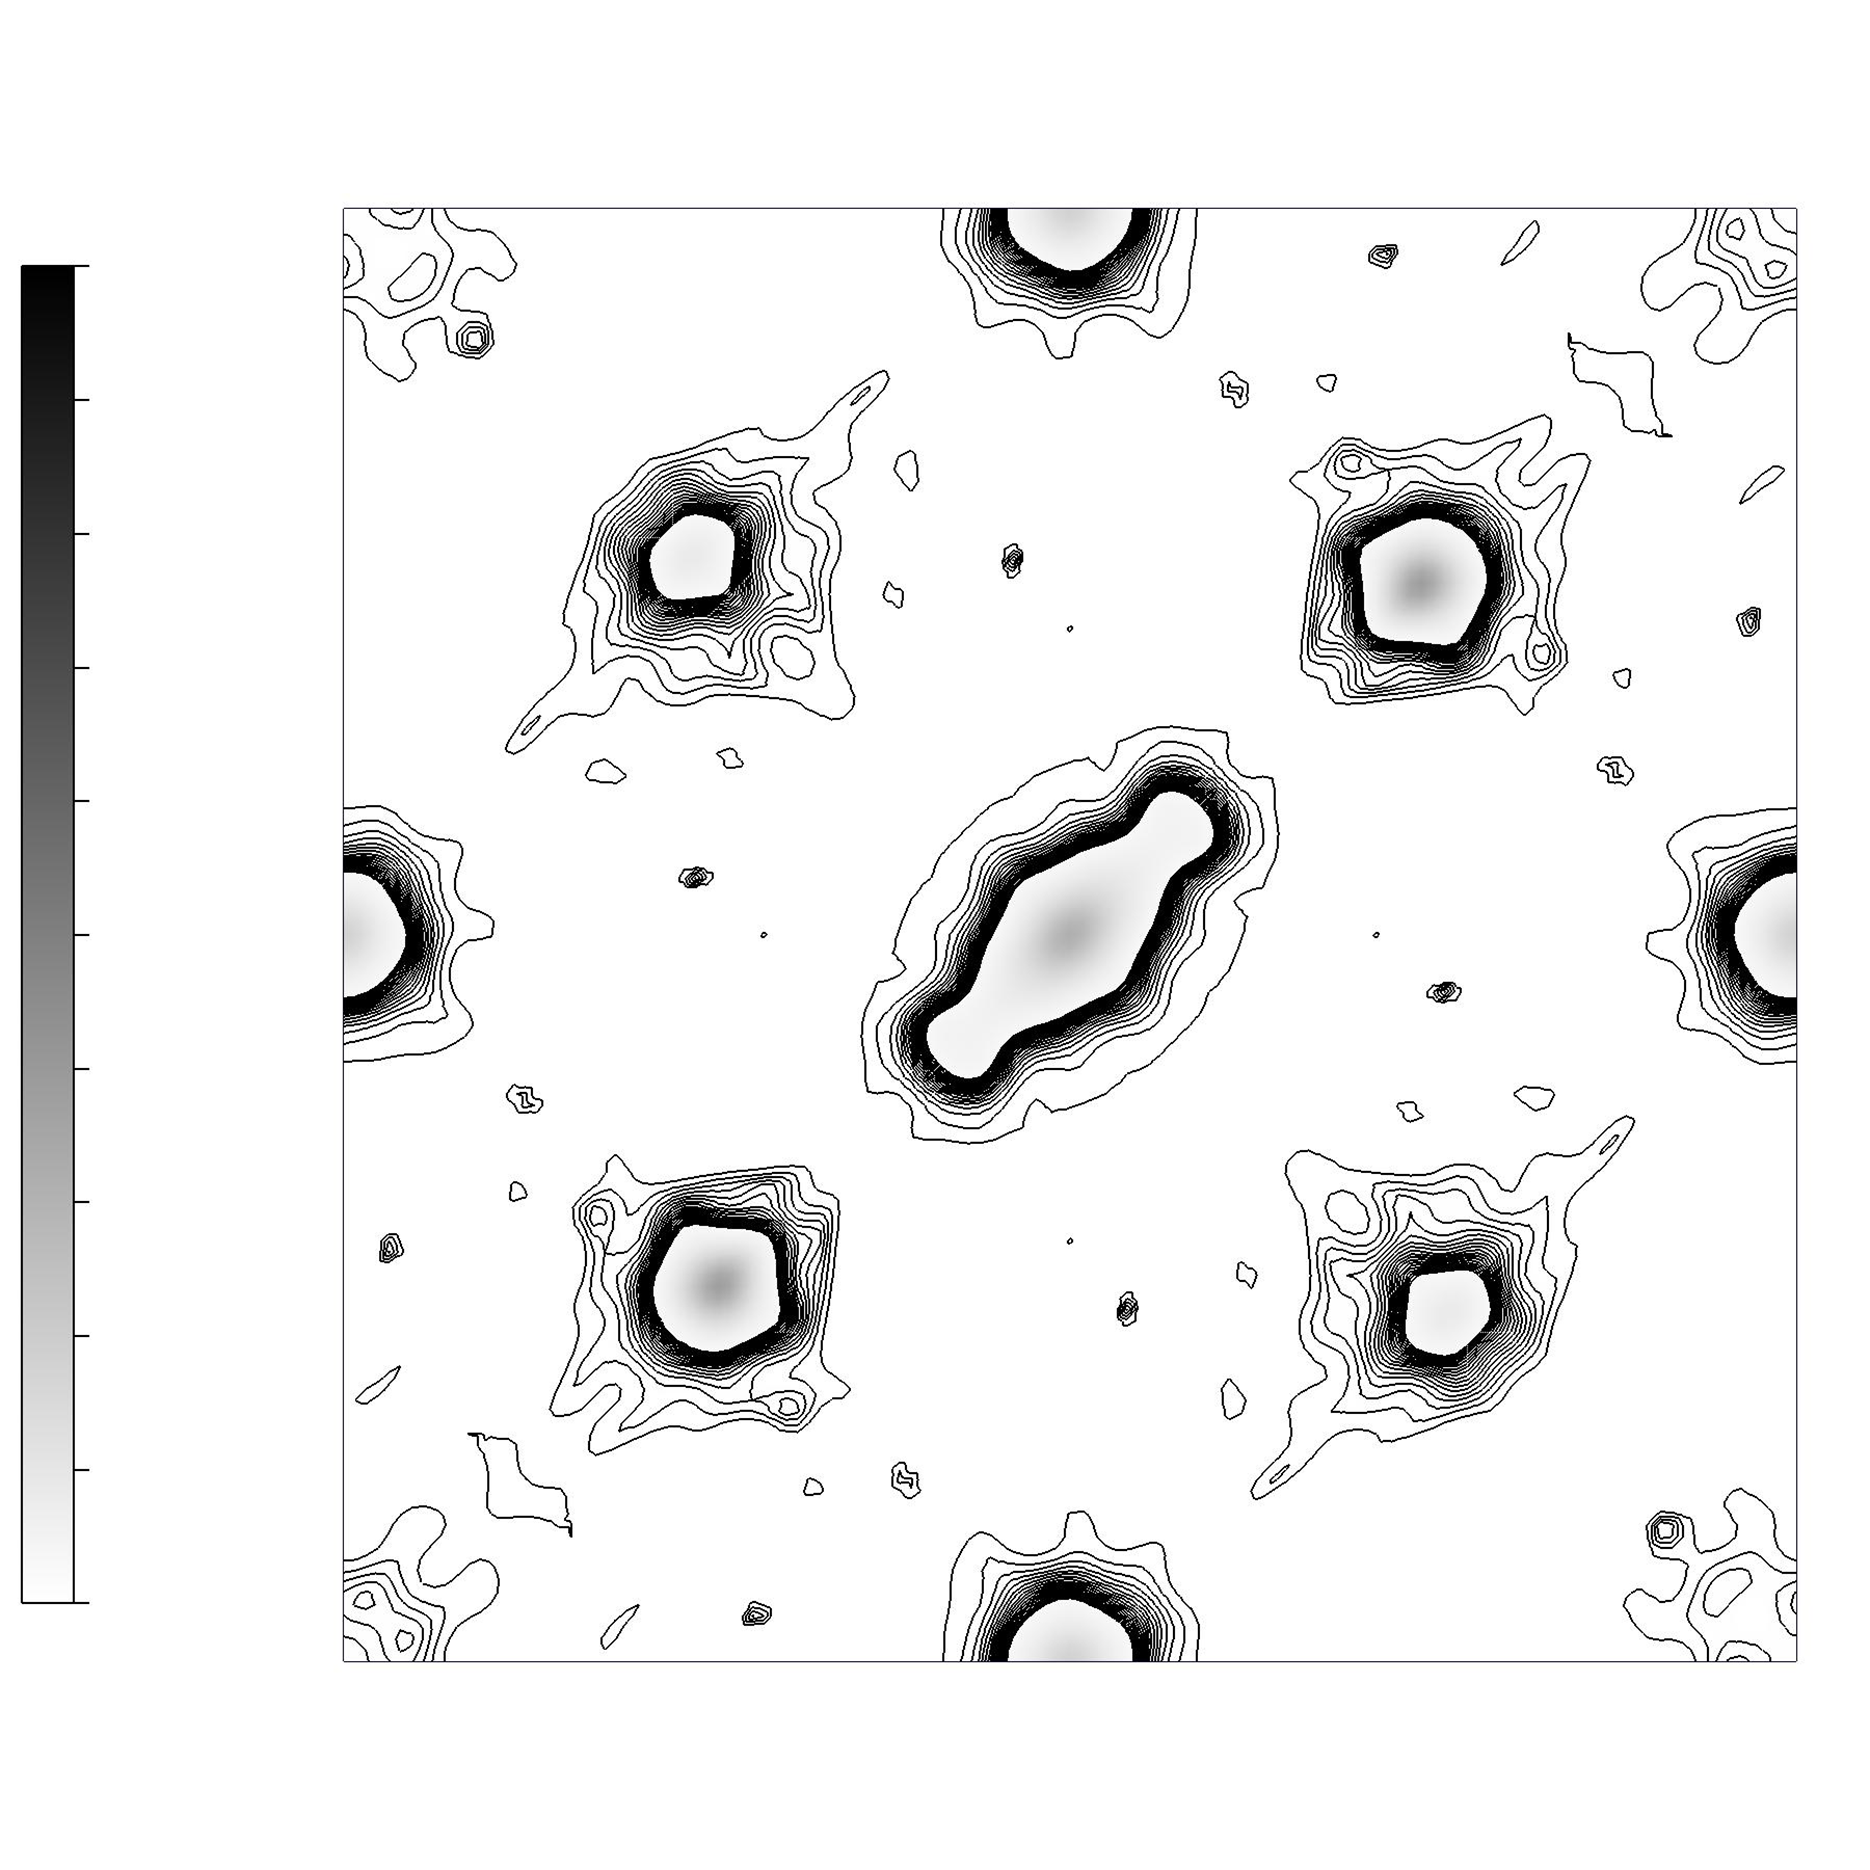
\includegraphics[width=0.9\linewidth]{Electron_density_As} \\ а)
 % \end{minipage}
 % \vfill
 % \begin{minipage}[ht]{0.7\linewidth}\centering
 %   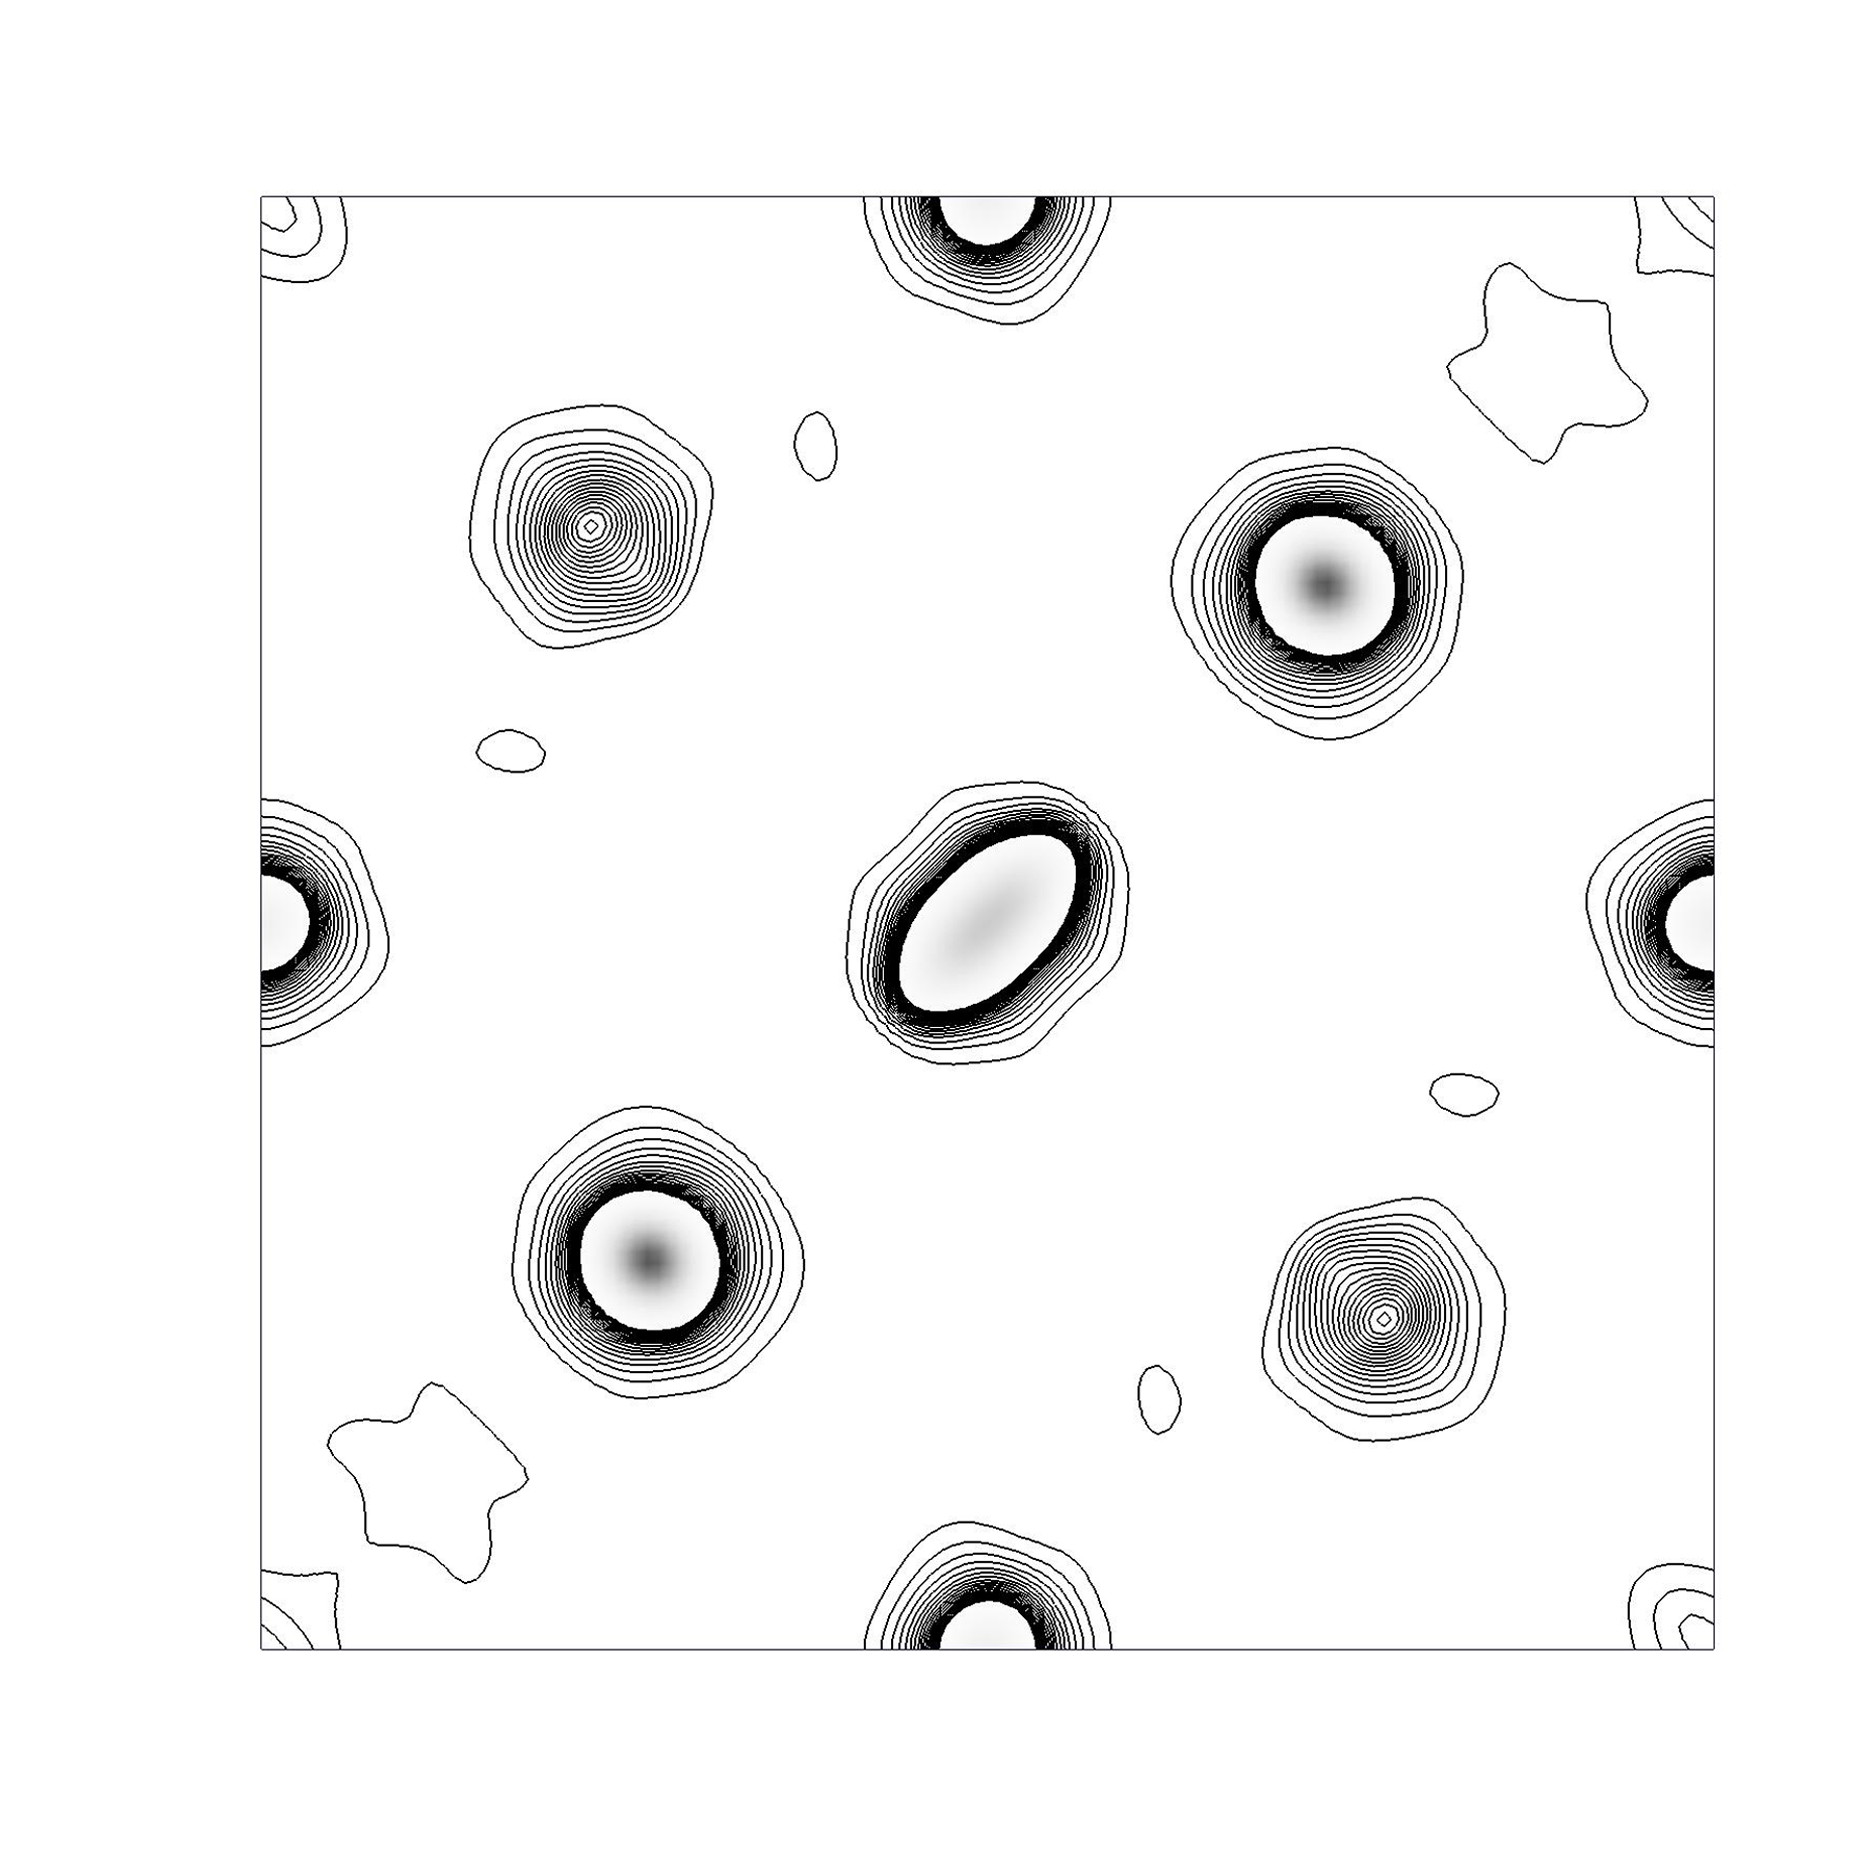
\includegraphics[width=0.9\linewidth]{Electron_density_Sb} \\ б)
 % \end{minipage}
 % \caption[Электронная плотность синтетического теннантита Cu\textsubscript{12}As\textsubscript{4}S\textsubscript{13} и тетраэдрита Cu\textsubscript{12}Sb\textsubscript{4}S\textsubscript{13}]{Электронная плотность синтетического теннантита Cu\textsubscript{12}As\textsubscript{4}S\textsubscript{13} и тетраэдрита Cu\textsubscript{12}Sb\textsubscript{4}S\textsubscript{13}}
  %  \label{img:figure2}
%\end{figure}



\begin{figure}[pt!]
\centering
  \begin{minipage}[ht]{0.7\linewidth}\centering
    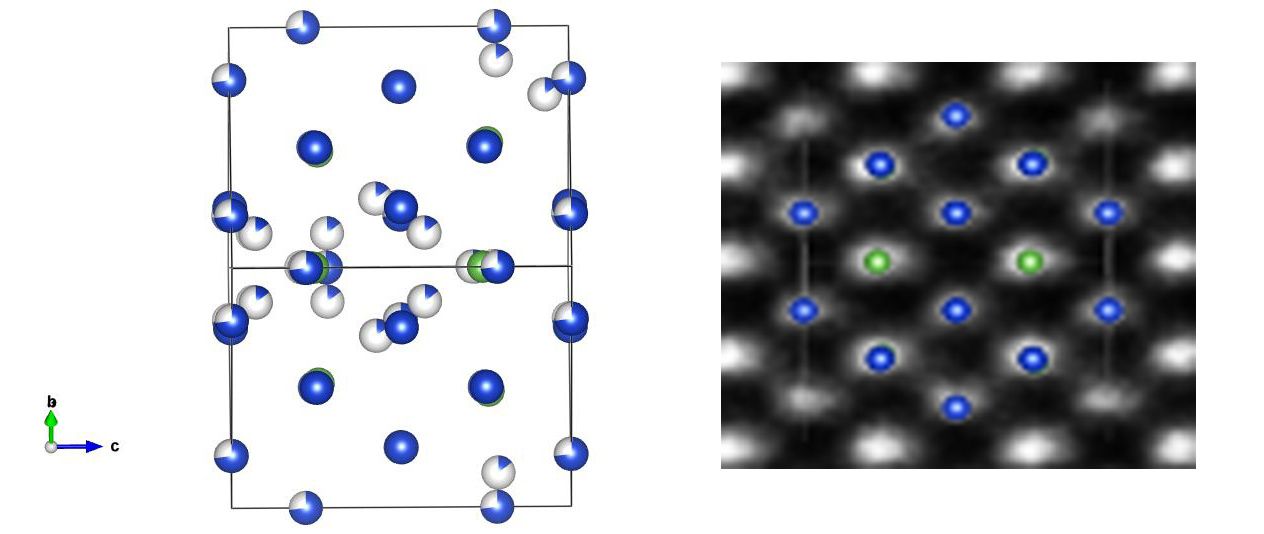
\includegraphics[width=0.9\linewidth]{mic_cu12as4s13_110} \\
  \end{minipage}

  \caption[HAADF изображение и теоретическая форма изображения рядов для образца Cu\textsubscript{12}As\textsubscript{4}S\textsubscript{13}]{HAADF изображение и теоретическая форма изображения рядов для образца Cu\textsubscript{12}As\textsubscript{4}S\textsubscript{13}}
    \label{img:mic3}
\end{figure}

\clearpage

\newpage

\section{Особенности теплоёмкости для образов Cu\textsubscript{12}As\textsubscript{4}S\textsubscript{13} и Cu\textsubscript{3}AsSe\textsubscript{3} } \label{sect3_2}

Данные об аномальном поведении теплоёмкости Cu\textsubscript{12}As\textsubscript{4}S\textsubscript{13} и Cu\textsubscript{3}AsSe\textsubscript{3} согласуются с опубликованными данными \cite{bab_1982,bab_81}.
В указанных работах в этих соединениях наблюдаются аномальное изменение магнитной восприимчивости, температурной зависимости коэффициента упругой податливости и отклонение от нормального хода температурной зависимости параметра кристаллической решетки.
Стоит отметить, что авторы работ \cite{bab_1982,bab_81} подразумевали наличие однофазных соединений и связывают наблюдаемые особенности с возникновением магнитного упорядочения на парамагнитных ионах Cu\textsuperscript{2+}.
Другие работы \cite{Lara-Curzio2014,Nasonova2016} на примере синтетического тетраэдрита рассматривают особенности транспортных свойств  с точки зрения наличия низкоэнергетических фононных мод в соединении. Наличие мод подтверждается на всех исследуемых в работе соединениях, что показано на рисунках \ref{img:raman1} и \ref{img:raman2}.
Авторами работ \cite{Lara-Curzio2014,Nasonova2016} установлено, что при температуре около 90 К происходит переход типа металл--полупроводник. Показано, что смещение атома серы, которое происходит вдоль поверхности октаэдра Cu\textsubscript{6}, и сдвиг атома меди, который осуществляется вдоль треугольника S\textsubscript{3}, связаны с увеличением расстояния между Cu--Sb.

\begin{figure}[p!]
  \begin{minipage}[ht]{0.9\linewidth}\centering
    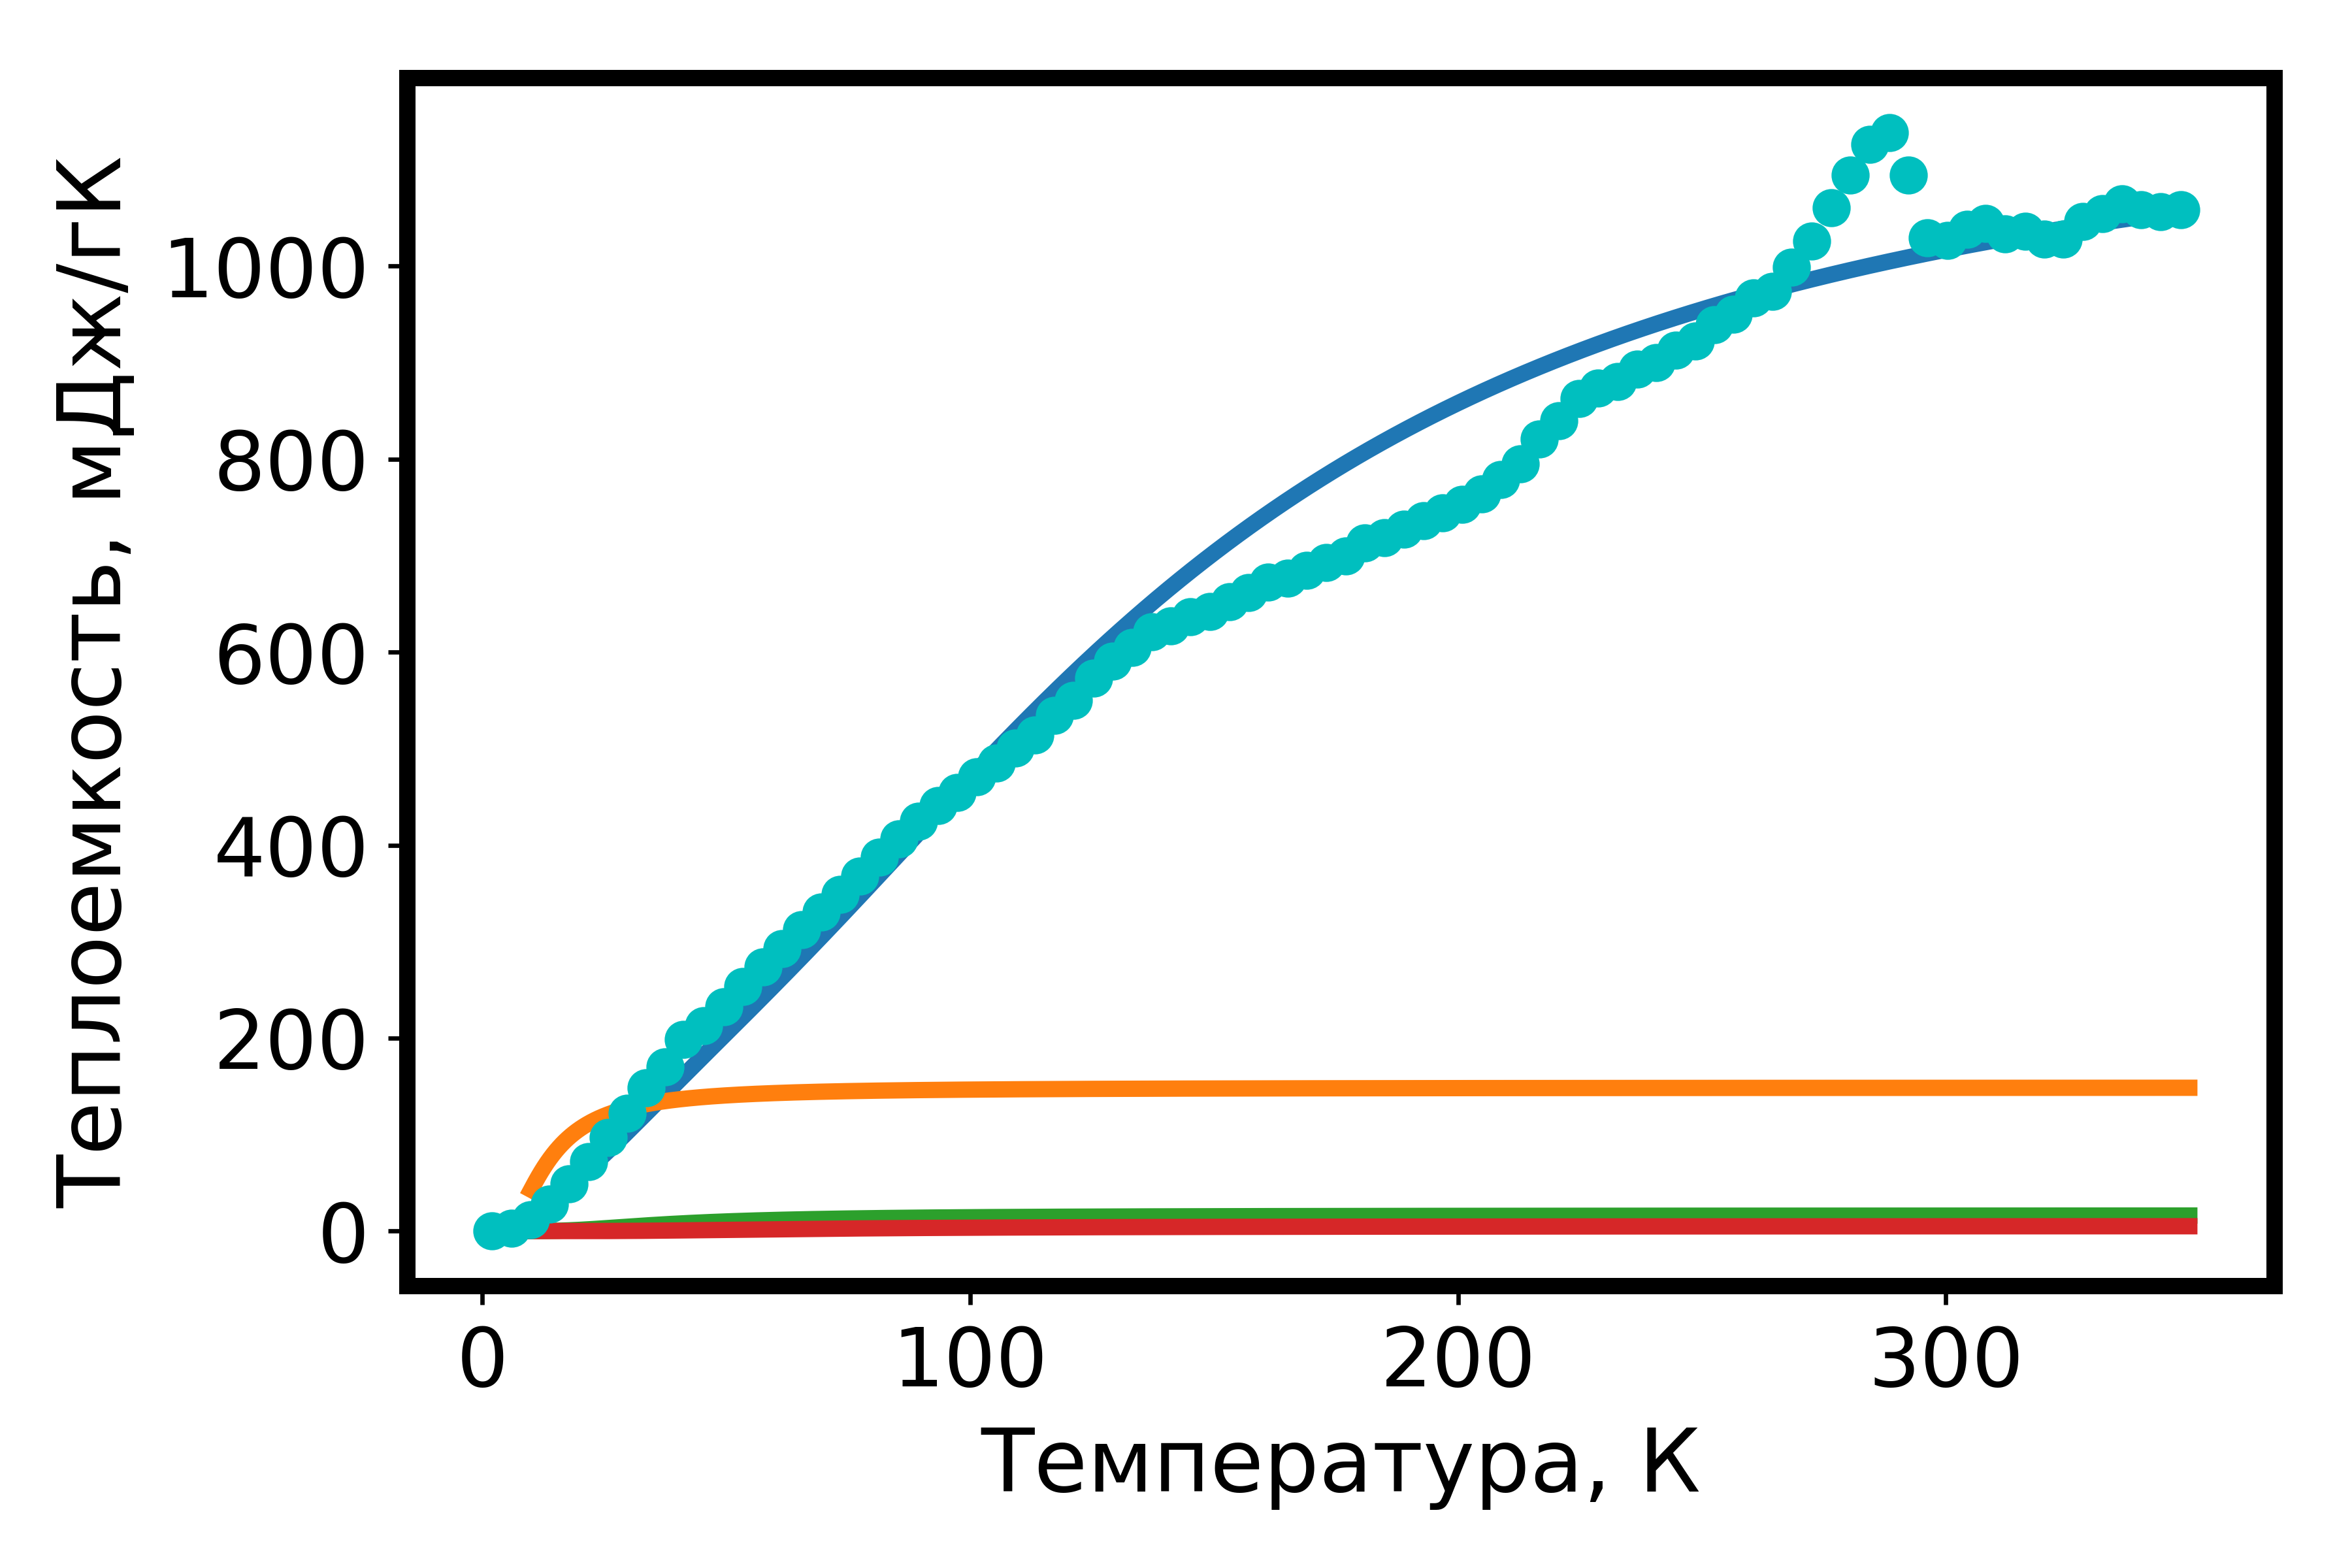
\includegraphics[width=0.9\linewidth]{Heat_capacity_cu12as4s13_with_eins} \\ а)
  \end{minipage}
  \vfill
  \begin{minipage}[ht]{0.9\linewidth}\centering
    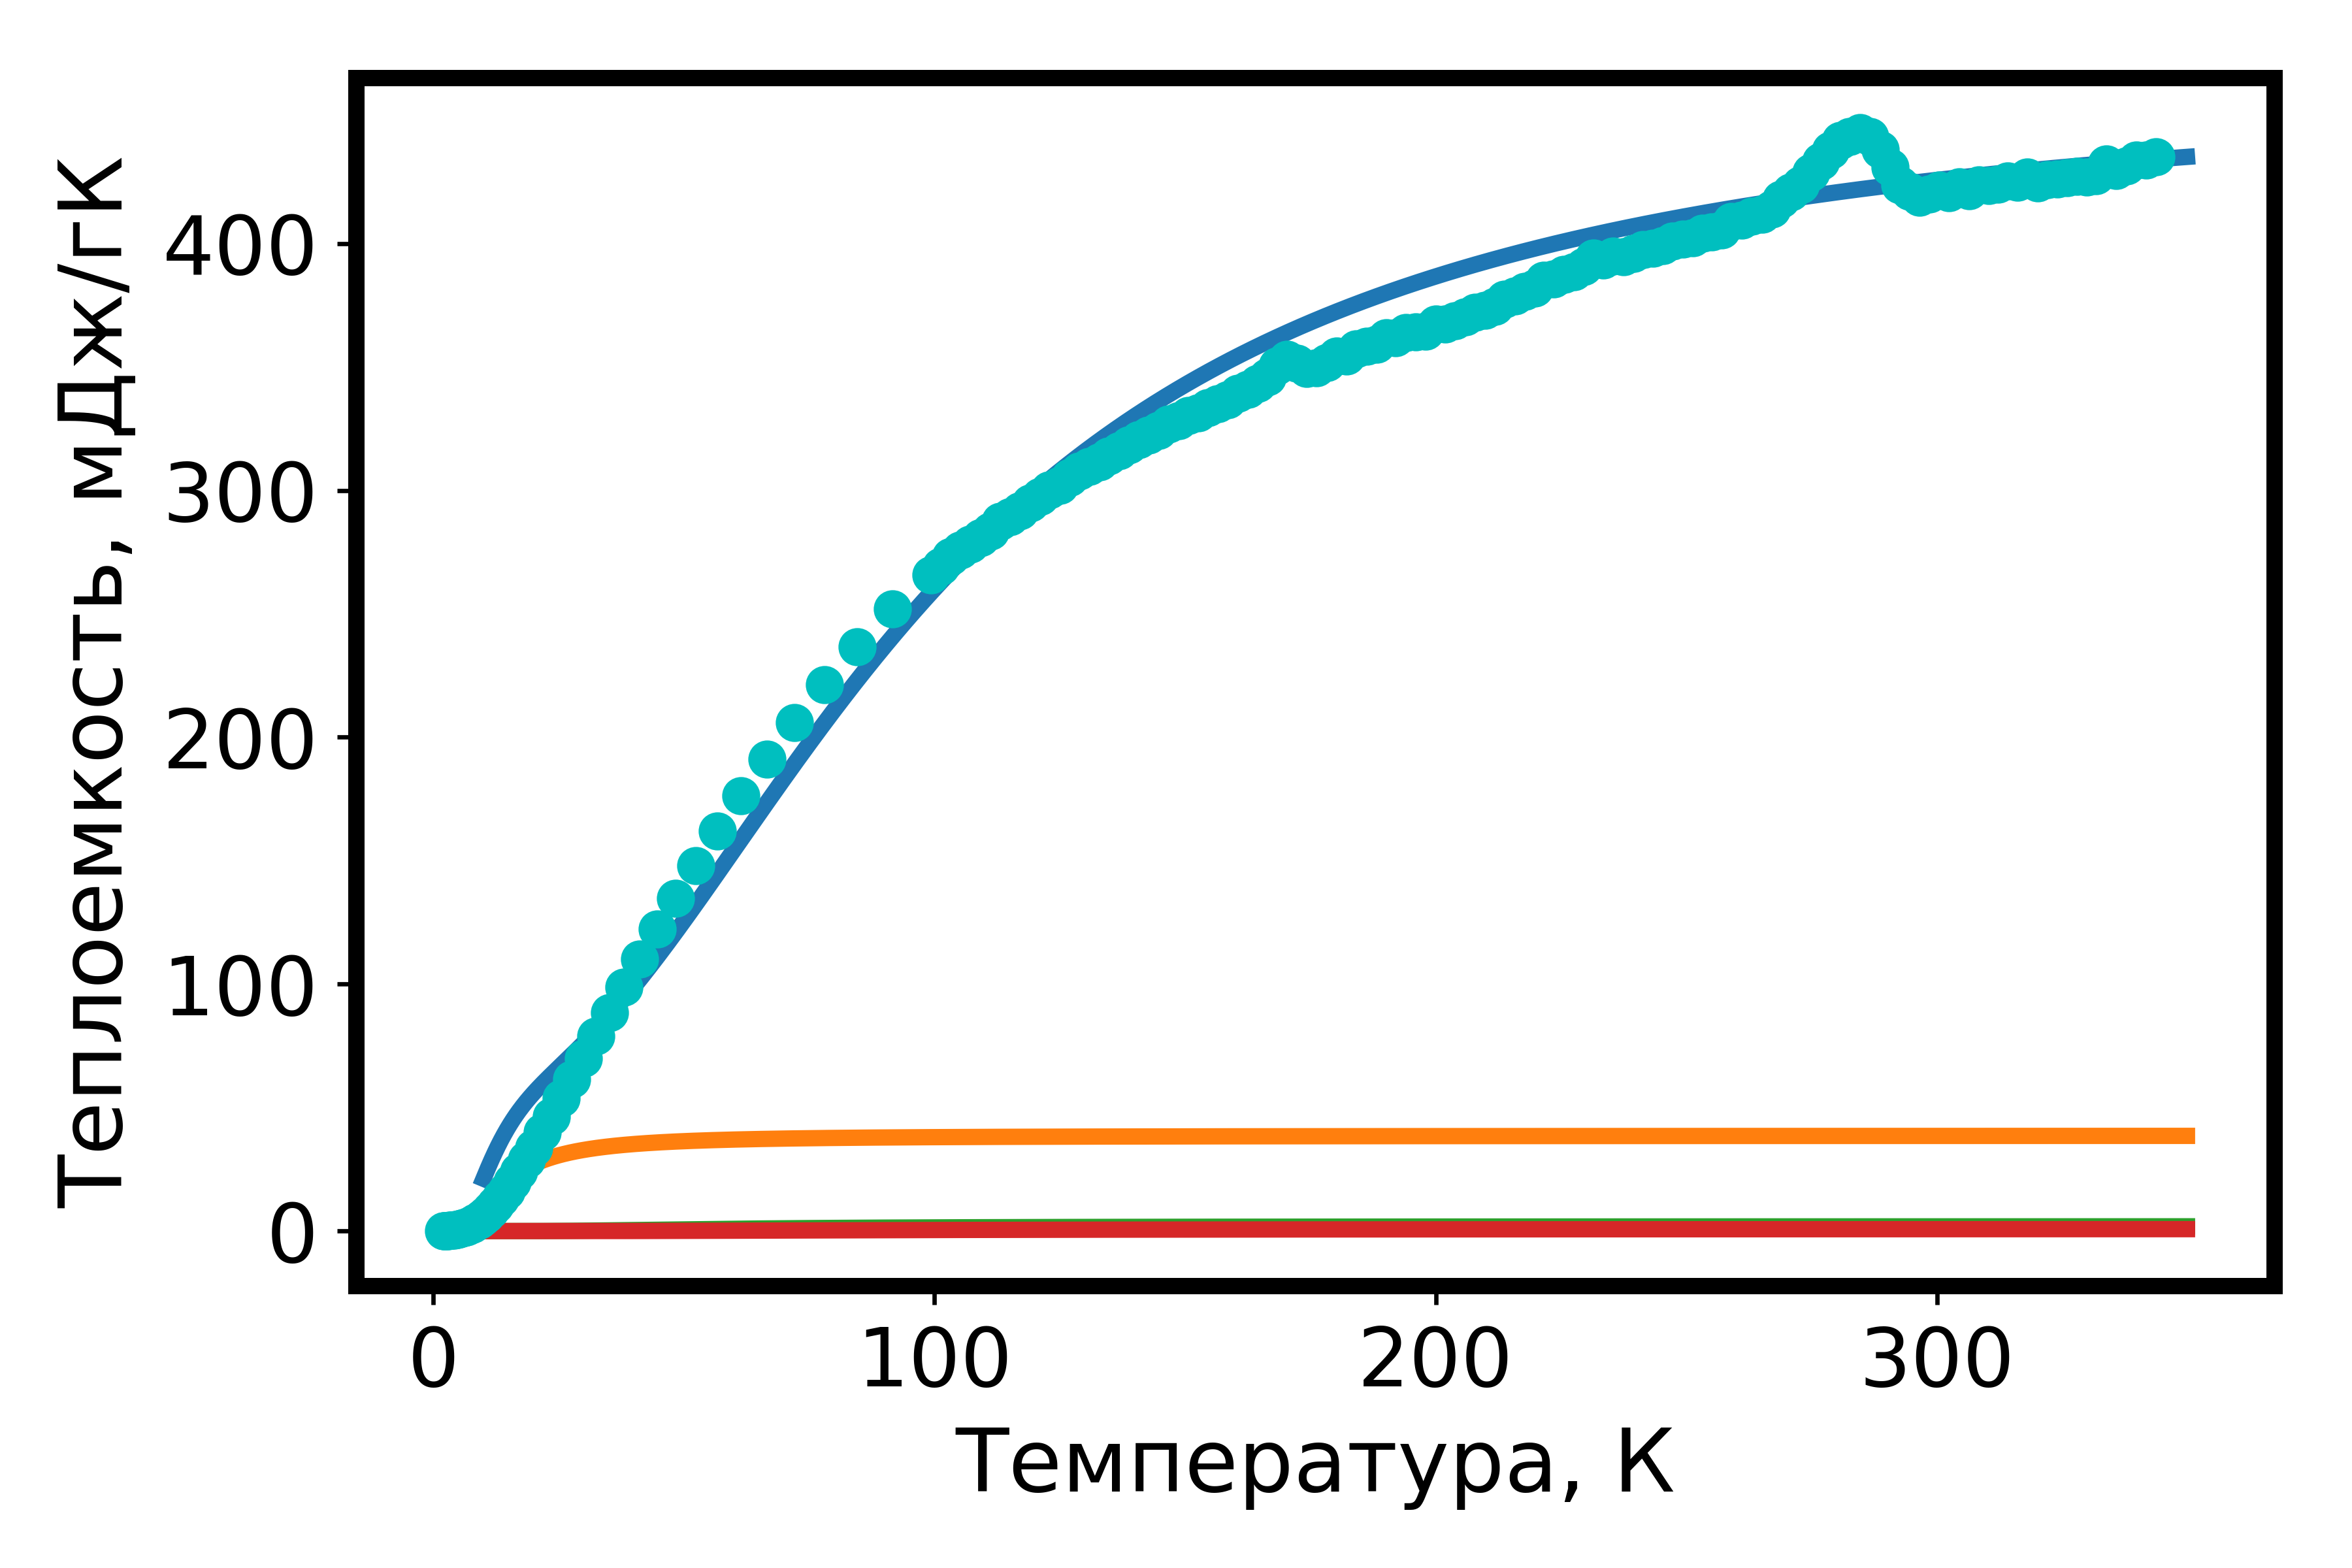
\includegraphics[width=0.9\linewidth]{Heat_capacity_cu3asse3_with_eins} \\ б)
  \end{minipage}

      \caption[Зависимость теплоёмкости образцов Cu\textsubscript{12}As\textsubscript{4}S\textsubscript{13}(а) и Cu\textsubscript{3}AsS\textsubscript{3}(б) от температуры. Точки "--- экспериментальные данные, сплошная линия "--- модельные значения теплоёмкости]{Зависимость теплоёмкости образцов Cu\textsubscript{12}As\textsubscript{4}S\textsubscript{13}(а) и Cu\textsubscript{3}AsS\textsubscript{3}(б) от температуры. Точки "--- экспериментальные данные, сплошная линия "--- модельные значения теплоёмкости}
    \label{img:heat_en}
\end{figure}


Авторы \cite{Lara-Curzio2014} отмечают, что фазовый переход в синтетическом тетраэдрите при 85~K значительно  влияет на транспортные свойства соединения: зарегистрировано резкое возрастание электрического сопротивления и максимум термоэлектрического выхода ниже фазового перехода. 
Особенности физических свойств объясняются наличием статистически разориентированной позицией меди Cu(II) в структуре тетраэдрита. Стоит отметить, что в температурном структурном эксперименте для теннантита позиции меди Cu2 и Cu21, заселённость которых изменяется с измениением температуры (Рис. \ref{img:xray}б), могут быть рассмотрены как статически разоентированные позиции меди Cu(II) в тетраэдрите.
Полученные в работе температурные  зависимости теплоёмкости обладают особенностями при тех же температурах, что и в опубликованных работах. 
Полученные экспериментальные зависимости описываются расчётной зависимостью теплоёмкости Дебая с дополнительными осцилляторами Эйнштейна.
Полученные подбором температуры Эйнштейна для теннантита согласуются со значениями температур Эйнштейна, полученных для атомов из структурного эксперимента.
Подобные дополнительные осцилляторы Эйнштейна, характеризующие смягчение фононных мод в кристалле\cite{bab_81}, позволяют описать полученную зависимость теплоёмкости.
По данным рентгеноструктурного анализа и квантовомеханического моделирования структура синтетического теннантита не обладает политипными модификациями. Таким образом, наблюдаемые аномалии в экспериментальных зависимостях теплоёмкостей, которые трактуются как смягчение фононных мод, представляют собой следствие суперпозиции фононных вкладов от атомов с высокими значениями коэффициентов атомарного смещения.
А наличие атомов с разными коэффициентами атомарного смещения может трактоваться, как возникновение спонтанной деформации\cite{bab_1982,bab_81}.
На рисунке \ref{img:heat_en} представлены зависимости расчётной и экспериментальной теплоёмкостей для  Cu\textsubscript{12}As\textsubscript{4}S\textsubscript{13} и Cu\textsubscript{3}AsS\textsubscript{3}.
Температура Дебая для Cu\textsubscript{12}As\textsubscript{4}S\textsubscript{13} составляет 623~К, а для Cu\textsubscript{3}AsS\textsubscript{3} "--- 500~К.
Дополнительно на каждом графике отмечены характерные температуры эйнштейновских осцилляторов, которые составляют 65, 124 и 220~К для Cu\textsubscript{12}As\textsubscript{4}S\textsubscript{13} и 42, 186 и 288~К для Cu\textsubscript{3}AsS\textsubscript{3}.
\clearpage

\newpage

\section{Закономерности изменения магнитных и некоторых физических свойств при изовалентном замещении в сложных халькогенидах меди} \label{sect3_3}

Все графики зависимостей магнитной восприимчивости обладают схожими особенностями при изменении температуры. Так, например, для соединения Cu\textsubscript{12}As\textsubscript{4}S\textsubscript{13} магнитное упорядочение происходит около 124~К, для Cu\textsubscript{3}AsSe\textsubscript{3} "--- около 170~К, для Cu\textsubscript{12}Sb\textsubscript{4}S\textsubscript{13}  "--- около 84~К и для Cu\textsubscript{3}SbSe\textsubscript{3}"--- около 170~К.

Согласно данным в работе \cite{Nasonova2016}, для синтетического теннантита и синтетического тетраэдрита, изменение магнитной восприимчивости вызвано изменением значения коэффициента атомного смещения для позиции S(2). Сдвиг температуры с 124 до 84~К упорядочения может быть вызван изменением локального окружения атома в позиции S(2) при изовалентном замещении As на Sb.
При подобном замещении в соединениях Cu\textsubscript{3}AsSe\textsubscript{3} и Cu\textsubscript{3}SbSe\textsubscript{3} аналогичного изменения не наблюдается. Этот факт может свидетельствовать о другом механизме фазового превращения или о многообразии возможных фазовых превращений в сложных халькогенидах меди ввиду наличия сложной ионно-ковалентной связи.
В литературе встречаются описание механизма антиферромагнитного упорядочения в сложных халькогенидах меди. Предположение о существовании антиферромагнитного упорядочения через Cu--S--Cu, вводится по аналогии с антиферромагнитным упорядочением Cu--O--Cu\cite{Crawford1976} c характерным $\phi$~=~96.94\textsuperscript{ $\circ$ }. По данным структурного исследования для синтетического теннантита в структуре возникает характерный $\phi$~=~96.01\textsuperscript{ $\circ$ } для Cu--S--Cu между позициями Cu21, S2 и Cu21. Также в литературе описывается механизм\cite{Gainov2008,Gainov_2006} перепрыгивания спина электрона между CuS\textsubscript{3} через S\textsubscript{2}, который допускает возможность возникновения магнитного упорядочения. По результатам экспериментов, проведенных в рамках диссертационной работы, не удаётся подтвердить или опровергнуть это предположение. По полученным данным структурного исследования синтетического теннантита можно заключить о неоднородности электронной плотности в структуре и, как следствие, наличии парамагнетизма.


Указанное совпадение говорит о том, что в кристаллической структуре образца существуют парамагнитные ионы, в роли которых могут выступать случайно расположенные атомы меди в двух- и одновалентных состояниях.

\begin{table} [htbp]%
    \centering
	\caption{Значение температуры плавления, плотности и микротвёрдости для сложных соединений халькогенидов меди}%
	\label{hard}% label всегда желательно идти после caption
    \renewcommand{\arraystretch}{1.5}
	\begin{tabular}{@{}@{\extracolsep{20pt}}lllll@{}}
        \toprule     %%% верхняя линейка
    	 & Cu\textsubscript{12}As\textsubscript{4}S\textsubscript{13} &Cu\textsubscript{3}AsSe\textsubscript{3}& Cu\textsubscript{12}Sb\textsubscript{4}S\textsubscript{13} &Cu\textsubscript{3}SbSe\textsubscript{3}	\\
        \midrule
    T\textsubscript{пл}, К & 893 & 880												& 773& 753	\\ \hline
    	$ \rho$, г/см 	&  4.78$\pm$0.02	 						& 4.96$\pm$0.02												&5.82$\pm$0.02 	& 6.41$\pm$0.02 \\ \hline
    	H $\times$10\textsuperscript{7}, Н/м\textsuperscript{-2} 	& 154$\pm$18	 						& 134$\pm$10 	& 127$\pm$20			& 82$\pm$8	\\ \hline

        \bottomrule
	\end{tabular}%
\end{table}
В таблице \ref{hard} показано, как при увеличении молекулярного веса, температуры плавления и микротвёрдость исследованных соединений уменьшается, а плотность исследованных соединений возрастает. Такое поведение может свидетельствовать об уменьшении сил межатомного взаимодействия и может быть связано с металлизацией химических
связей.

Показано, что для получения соединения Cu\textsubscript{12}V\textsubscript{4}VI\textsubscript{13} предпочтительным является синтез из
исходной шихты с избытком по легколетучему компоненту, с последующей закалкой и
дополнительным отжигом в течении 120 часов при температуре 500 К.
\clearpage

\newpage
